\section{14 de enero de 2021}
\begin{remark}
Como el valor absoluto de $|a|\geq 0\to -|a|\leq |a|\to -|a|\leq a\leq|a|, \forall a $
\end{remark}

\begin{theorem}[Desigualdad triangular]
Sea $a$ y $b$ elementos de un campo ordenado $\mathbb{F}$. Entonces $|a+b|\leq |a|+|b|$
\end{theorem}
\begin{proof}
\begin{align}
    -|a|\leq & a \leq |a|\\
    -|b|\leq & b \leq |b|\\
    -(|a|+|b|)\leq & a+b \leq |a|+|b|\\
    |a+b|\leq & |a|+|b|
\end{align}
\end{proof}

\begin{remark}
Si $a,b$ son elementos del campo ordenado $F$, entonces: 
\begin{itemize}
    \item 
    \begin{align}
    ||a|-|b|| & \leq |a-b|
    \intertext{En efecto:}
    |a|= |(a-b)+b|\leq |a-b|+|b|\\
    \to |a|-|b|\leq |a-b|
    \intertext{Por otro lado:}
    |b|= |(b-a)+a|\leq |b-a|+|a|\\
    \to |b|-|a|\leq |b-a|=|a-b|\\
    \to ||a|-|b||\leq |a-b|
    \end{align}
    \item Si sustituimos $b$ por $-b$ en $(1)$
    \begin{align}
        \to ||a|-|b||\leq |a-(-b)|\\
        \to ||a|-|b||\leq |a+b|
    \end{align}
    \item Si sustituimos en (*) $b$ por $-b$ se tiene: 
    \begin{align}
        |a+(-b)|\leq |a|+|-b|\\
        \to |a-b|\leq |a|+|b|
        \intertext{Conclusión:}
        ||a|-|b||\leq |a\pm b|\leq |a|+|b| \textit{ (Desigualdad triangular)}
    \end{align}
\end{itemize}
\end{remark}

\subsubsection{Propiedad arquímedeada (o de Arquímedes)}
\begin{definition}
Un campo ordenado $\mathbb{F}$ es arquimedeano si $\forall x \in \mathbb{F}\exists n\in \mathbb{Z}^+\ni x<n$.
\end{definition}

\begin{remark}
La clase positiva $P$ de $\mathbb{F}$ es arquimediana si $\forall x\in \mathbb{F}\exists \mathbb{Z}^+\ni n-x\in P.$ 
\end{remark}

\begin{kaobox}[frametitle=Ejercicios]
\begin{enumerate}
    \item Compruebe que el campo $\mathbb{Q}$ es arquimeadeano. 
    \begin{itemize}
        \item ¿Depende este enunciado del orden que se defina en $\mathbb{Q}$?
    \end{itemize}
    \item Presente un ejemplo de un campo ordenado que sea arquimediano. 
\end{enumerate}
\end{kaobox}

\begin{theorem}
Si $\mathbb{F}$ es un campo arquimedeano, entonces: 
\begin{itemize}
    \item Si $y>0$ y $z>0\to\exists n\in \mathbb{Z}^+\ni ny>z$
    \item Si $z>0\to \exists n \in \mathbb{Z}^+\ni 0<\frac{1}{n}<z$
    \item Si $y>0\to \exists n \in \mathbb{Z}^+\ni n-1\leq y< n$
\end{itemize}
\end{theorem}

\begin{proof}
...
\begin{enumerate}
    \item Si $y>0$ y $z>0\ni x:=\frac{z}{y}>0\to \exists n\in \mathbb{Z}^+\ni n>\frac{z}{y}\to ny>z$
    \item Si $z>0\to \frac{1}{z}>0\to \exists n \in \mathbb{Z}^+\ni n>\frac{1}{z}\to \frac{1}{n}<z\to  0<\frac{1}{n}<z$
    \item Sea $y>0\to\exists m\in \mathbb{Z}^+\ni y<m.$
    \begin{center}
        

\tikzset{every picture/.style={line width=0.75pt}} %set default line width to 0.75pt        

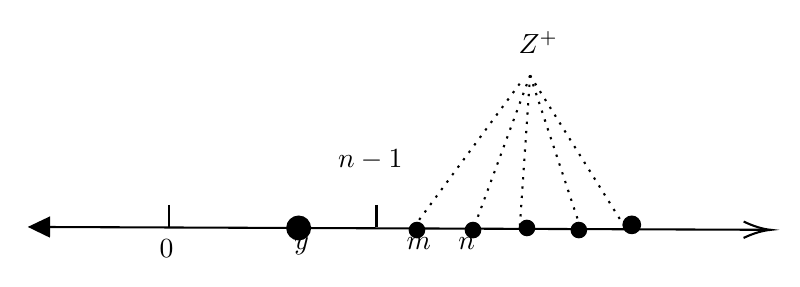
\begin{tikzpicture}[x=0.75pt,y=0.75pt,yscale=-1,xscale=1]
%uncomment if require: \path (0,300); %set diagram left start at 0, and has height of 300

%Straight Lines [id:da34781333711164497] 
\draw    (135,152.01) -- (488,153.39) ;
\draw [shift={(490,153.4)}, rotate = 180.22] [color={rgb, 255:red, 0; green, 0; blue, 0 }  ][line width=0.75]    (13.12,-3.95) .. controls (8.34,-1.68) and (3.97,-0.36) .. (0,0) .. controls (3.97,0.36) and (8.34,1.68) .. (13.12,3.95)   ;
\draw [shift={(132,152)}, rotate = 0.22] [fill={rgb, 255:red, 0; green, 0; blue, 0 }  ][line width=0.08]  [draw opacity=0] (10.72,-5.15) -- (0,0) -- (10.72,5.15) -- cycle    ;
%Straight Lines [id:da8197597860941424] 
\draw    (200,141.4) -- (200,152) ;
%Shape: Circle [id:dp09256163312530119] 
\draw  [fill={rgb, 255:red, 0; green, 0; blue, 0 }  ,fill opacity=1 ] (257,152.5) .. controls (257,149.46) and (259.46,147) .. (262.5,147) .. controls (265.54,147) and (268,149.46) .. (268,152.5) .. controls (268,155.54) and (265.54,158) .. (262.5,158) .. controls (259.46,158) and (257,155.54) .. (257,152.5) -- cycle ;
%Shape: Circle [id:dp6277393793069347] 
\draw  [fill={rgb, 255:red, 0; green, 0; blue, 0 }  ,fill opacity=1 ] (323,153.5) .. controls (323,151.57) and (321.43,150) .. (319.5,150) .. controls (317.57,150) and (316,151.57) .. (316,153.5) .. controls (316,155.43) and (317.57,157) .. (319.5,157) .. controls (321.43,157) and (323,155.43) .. (323,153.5) -- cycle ;
%Straight Lines [id:da8933443153155035] 
\draw    (300,141.4) -- (300,152) ;
%Shape: Circle [id:dp3886664444977367] 
\draw  [fill={rgb, 255:red, 0; green, 0; blue, 0 }  ,fill opacity=1 ] (350,153.5) .. controls (350,151.57) and (348.43,150) .. (346.5,150) .. controls (344.57,150) and (343,151.57) .. (343,153.5) .. controls (343,155.43) and (344.57,157) .. (346.5,157) .. controls (348.43,157) and (350,155.43) .. (350,153.5) -- cycle ;
%Shape: Circle [id:dp7285230821464551] 
\draw  [fill={rgb, 255:red, 0; green, 0; blue, 0 }  ,fill opacity=1 ] (376,152.5) .. controls (376,150.57) and (374.43,149) .. (372.5,149) .. controls (370.57,149) and (369,150.57) .. (369,152.5) .. controls (369,154.43) and (370.57,156) .. (372.5,156) .. controls (374.43,156) and (376,154.43) .. (376,152.5) -- cycle ;
%Shape: Circle [id:dp05916074085979284] 
\draw  [fill={rgb, 255:red, 0; green, 0; blue, 0 }  ,fill opacity=1 ] (401,153.5) .. controls (401,151.57) and (399.43,150) .. (397.5,150) .. controls (395.57,150) and (394,151.57) .. (394,153.5) .. controls (394,155.43) and (395.57,157) .. (397.5,157) .. controls (399.43,157) and (401,155.43) .. (401,153.5) -- cycle ;
%Shape: Circle [id:dp7010184215808682] 
\draw  [fill={rgb, 255:red, 0; green, 0; blue, 0 }  ,fill opacity=1 ] (427,151) .. controls (427,148.79) and (425.21,147) .. (423,147) .. controls (420.79,147) and (419,148.79) .. (419,151) .. controls (419,153.21) and (420.79,155) .. (423,155) .. controls (425.21,155) and (427,153.21) .. (427,151) -- cycle ;
%Straight Lines [id:da16881291068353932] 
\draw  [dash pattern={on 0.84pt off 2.51pt}]  (369,83) -- (319.5,150) ;
%Straight Lines [id:da5836547700471342] 
\draw  [dash pattern={on 0.84pt off 2.51pt}]  (374,79) -- (346.5,153.5) ;
%Straight Lines [id:da027764970183191462] 
\draw  [dash pattern={on 0.84pt off 2.51pt}]  (374,79) -- (369,152.5) ;
%Straight Lines [id:da432529211764785] 
\draw  [dash pattern={on 0.84pt off 2.51pt}]  (374,79) -- (397.5,150) ;
%Straight Lines [id:da9746308185178715] 
\draw  [dash pattern={on 0.84pt off 2.51pt}]  (374,79) -- (419,151) ;

% Text Node
\draw (280,113.5) node [anchor=north west][inner sep=0.75pt]    {$n-1$};
% Text Node
\draw (194,156.5) node [anchor=north west][inner sep=0.75pt]    {$0$};
% Text Node
\draw (259,155.6) node [anchor=north west][inner sep=0.75pt]    {$y$};
% Text Node
\draw (313,155.8) node [anchor=north west][inner sep=0.75pt]    {$m$};
% Text Node
\draw (338,155.5) node [anchor=north west][inner sep=0.75pt]    {$n$};
% Text Node
\draw (367,56.5) node [anchor=north west][inner sep=0.75pt]    {$\mathbb{Z}^{+}$};


\end{tikzpicture}
    \end{center}
    \marginnote[-12   pt ]{En matemática, el teorema del buen orden establece que todo conjunto puede ser bien ordenado. Un conjunto X está bien ordenado por un orden estricto si todo subconjunto no vacío de X tiene un elemento mínimo bajo dicho orden. También se conoce como teorema de Zermelo y es equivalente al axioma de elección.}
    Sea $n$ el menor de tales enteros positivos $m$ ($n$ existe por el principio del buen orden). Entonces, $n-1\leq y < n$. 
\end{enumerate} 
\end{proof}

\begin{remark}[Cota superior más pequeña]
Sea $B\subset \mathbb{Q}, B\neq \mathbb{Q}$. Entonces, $B$ es acotado superiormente, si $k\in \mathbb{Q}$. Entonces, $B$ es acotado superiormente si $k\in \mathbb{Q}\ni k\geq b, \forall b\in B$. (En este caso $k$ es cota superior de $B$. 
\end{remark}

\begin{example}
\begin{enumerate}
    \item Sea $\s{a\in \mathbb{Q}\to a<4}$ (este conjunto está acotado superiormente por 4 [pero también 5, 16,... son cotas superiores.]). Por otro lado, $\mathbb{N} \leq \mathbb{Q}$ no es acotado. 
    \item Si $B\subset \mathbb{Q}, B\neq \mathbb{Q}$ y $B$ es acotado superiormente, entonces la cota superior más pequeña de $B$ es un número $k\in \mathbb{Q}\ni$
    \begin{itemize}
        \item $k$ es cota superior.
        \item si $C$ es cota superior de $B$, entonces $C\geq k$. 
    \end{itemize}
    \item Si existe la cota superior más pequeña de $B$, esta es única. \newline 
    Suponga que $k_1$ y $k_2$ son las cotas superiores más pequeñas de $B$. Entonces
    \begin{itemize}
        \item Como $k_1$ es cota superior más pequeña y $k_2$ es cota superior $k_2\geq k_1$. 
        \item Como $k_2$ es cota superior más pequeña y $k_1$ es cota superior $\to k_1\geq k_2\to k_1=k_2$
    \end{itemize}
    \item Considere el conjunto $c=\s{a\in \mathbb{Q}: a\geq 0 \text{ y } a<2}$ Nótese que $C$ está acotado superiormente. En efecto, si $a\in C\to a^2<4\to a<2\to 2$ es cota superior de $C$. 
    \item ¿Es 2 la menor cota superior de $C$? No, considere: $a^2 < -\frac{a}{4}\to a<\frac{3}{2}=1.5$
\end{enumerate}
\end{example}

\begin{kaobox}[frametitle=Para investigar]
\begin{itemize}
    \item Cotas superiores.
    \item Supremo de dos conjuntos = Cota superior. 
\end{itemize}
\end{kaobox}

